\section{Scalability evaluation}
\label{sec:evaluation}


The purpose of this section is to quantify the scalability of
our  framework. In this context, the adaptation to small streams is irrelevant so we disable it.
%
Our implementation extends the code in Apache DataSketches (Incubating)~\cite{DataSketches}, a Java
open-source library of stochastic streaming algorithms. The $\Theta$ sketch implementation there
differs slightly from the KMV $\Theta$ sketch we  used as a running example, and is
based on a HeapQuickSelectSketch family. In this version, the sketch stores between $k$ and $2k$ items
whilst keeping $\Theta$ as the $k^{th}$ largest value. When the sketch is full,
it is sorted and largest $k$ values are discarded. 

We experimented on a dedicated machine with four Intel
Xeon E5-4650 processors, each with $8$ cores, for a total of
$32$ threads (with hyper-threading disabled).
We ran an \emph{update-only} workload in
which a sketch is built from a very large stream. Repeated experiments showed similar results. 


\begin{figure}[tb]
\setlength{\abovecaptionskip}{0pt}
\setlength{\belowcaptionskip}{0pt}
\setlength\textfloatsep{0pt}
%\begin{wrapfigure}{r}{0.45\textwidth}
  \begin{center}
    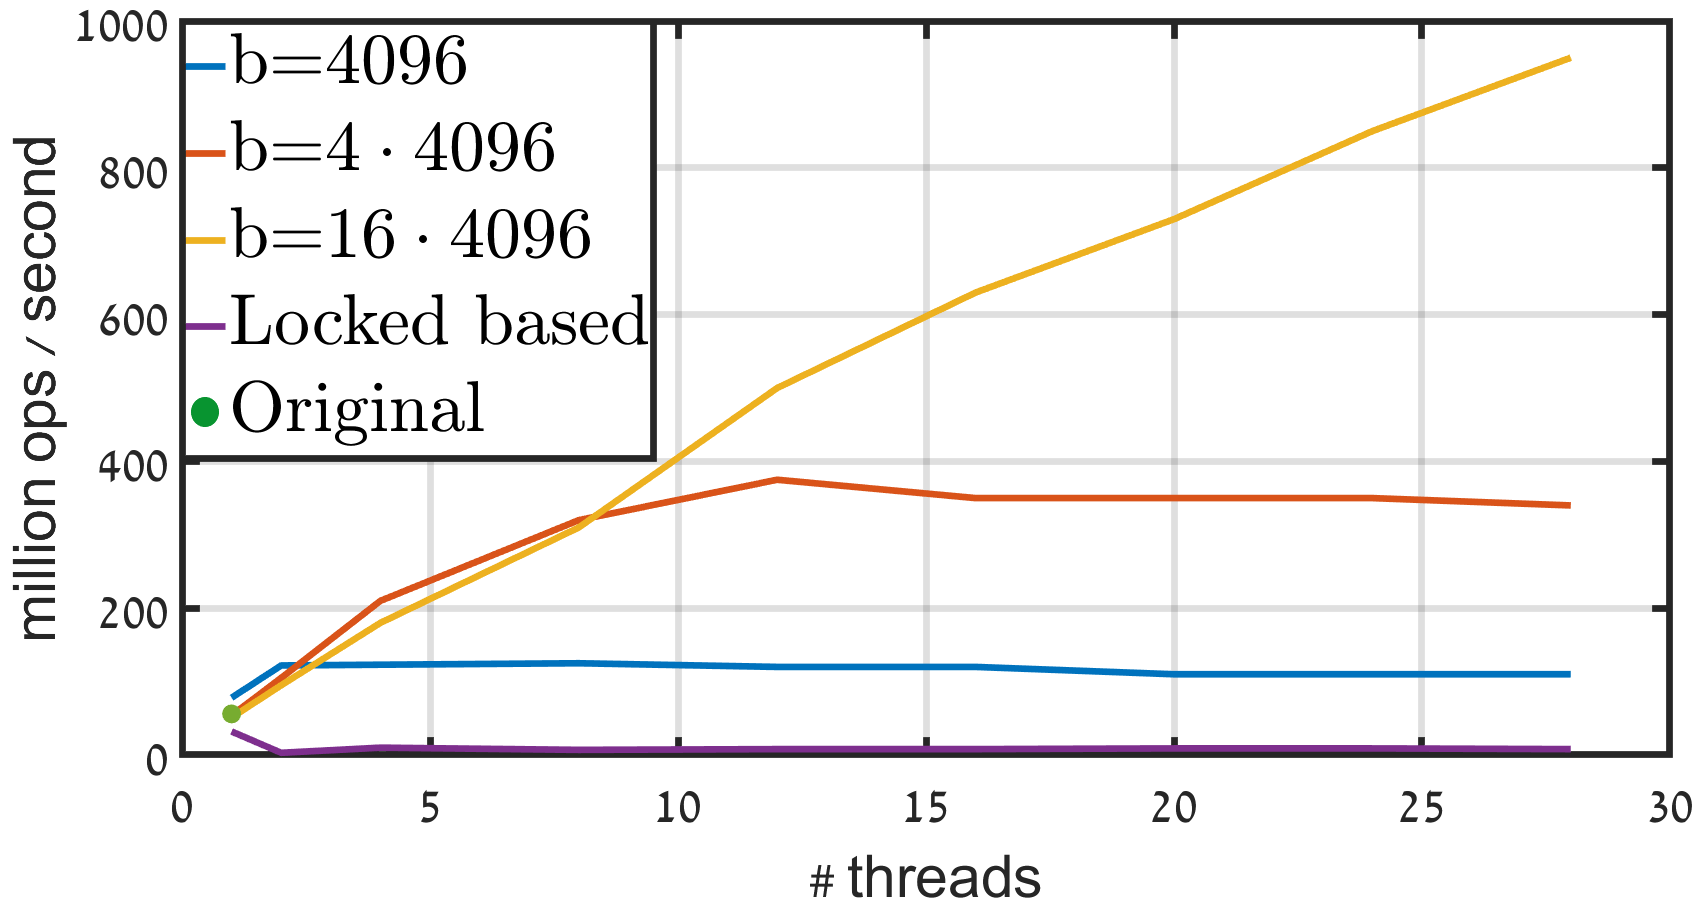
\includegraphics[width=0.44\textwidth]{images/QuantilesUpdate.png}
  \end{center}
  \caption{Scalability of DataSketches' Quantiles sketch 
  protected by a lock vs. our concurrent implementation with different local
  buffer sizes $b$.}
      \label{fig:ConccurentQuantilesUpdate}
%\end{wrapfigure}
\end{figure}





Our baselines are the sequential sketches
from the library, wrapped with a read/write lock
to allow concurrency. Our results show that adding the lock reduces
the single-thread performance of the $\Theta$ sketch
from 90 to 32 million operations per second, and that of the Quantiles
sketch from 77 to 32 million.

In Figure~\ref{fig:performance} (in the introduction) we compare the scalability
of our concurrent $\Theta$ sketch and the original sketch wrapped
with a read/write lock in an update-only workload, for $b=16$ and $k=4096$.
As expected, the lock-based sequential sketch does not scale, and
in fact it performs worse when accessed concurrently by many
threads.
In contrast, our sketch achieves almost perfect scalability.
We also tried smaller local buffers, as small as $b=1$,
and the results were similar; for large streams $\Theta$ sketch
is not sensitive to the buffer size thanks to using shouldAdd to
prune out updates. $\Theta$ quickly
becomes small enough to allow filtering out most of the updates and so even small
local buffers fill up slowly.

Our concurrent Quantiles' snapshot method uses a double collect
on a dedicated \emph{bitmap} variable in the sketch library. This sketch
does not use hints: calcHint returns 1 and shouldAdd always returns true.

In Figure~\ref{fig:ConccurentQuantilesUpdate} we compare the
throughput of our Quantiles sketch to the baseline.
We see that again the baseline achieves the best result with a single worker thread.
Our sketch, in contrast, scales perfectly when every thread
has a sufficiently large local buffer.
But here, in order for the
background thread to support more worker threads, we have to
enlarge the local buffers. This is because, unlike $\Theta$,
we do not use a hint to reduce the frequency of updates to local buffers.